%This is chapter 2
%%=========================================
\chapter{Theoretical basis}

%%=========================================
\section{JavaScript}

Some relevant text

\subsection{Interpreter}
More text. \\
And a Formula:
\begin{equation}
V=W\times L\times D
\label{eq1}
\end{equation}
and another
\begin{equation}
F_{buoyancy}=V\times \rho\times g
\label{eq1}
\end{equation}

And a reference to a clever researchers paper \citep{hydrodynamics}.

\subsection{Topic 1.2}
Adding a figure that is scaled
\begin{figure}[h]
\centering
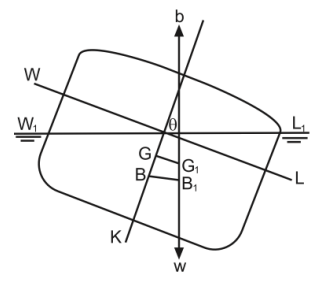
\includegraphics[scale=0.8]{fig/AngleOfList}
\caption{Angle of list.}
\label{fig1}
\end{figure}

\subsection{Topic 1.3} \label{stability}
Stability is a ships ability to right it self. 
A ship can also have a stable angle of list, meaning that the angle do not change. If a force has made the ship to roll, it will return to the same angle of list.

\subsubsection{Topic 1.3.1}
The Meta centre is the point the buoyancy force crosses the vessels centre line.
At small angles the vessel will rotate around this point.
In this case a small angle is less then 10\degree. 
At larger angles the meta centre will start to move, and the stability will no longer be linear.

\subsubsection{Topic 1.3.2}
Centre of gravity is the average location of the weight of an object and has the notation G.
See figure \ref{press}


And a table:

\begin{table}[H]
\centering
\caption{The notation of SNAME (1950) for marine vessels \citep{hydrodynamics}}
\label{my-label}
\begin{tabular}{|l|l|l|c|c|}
\hline
DOF &                                         & \begin{tabular}[c]{@{}l@{}}Forces and\\ moments\end{tabular} & \multicolumn{1}{l|}{\begin{tabular}[c]{@{}l@{}}Linear and\\ angular velocities\end{tabular}} & \multicolumn{1}{l|}{\begin{tabular}[c]{@{}l@{}}Positions and\\  Euler angles\end{tabular}} \\ \hline
1   & motions in the x direction (surge)      & X                                                            & \textit{u}                                                                                   & \textit{x}                                                                                 \\ \hline
2   & motions in the y direction (sway)       & Y                                                            & \textit{v}                                                                                   & \textit{y}                                                                                 \\ \hline
3   & motions in the z direction (heave)      & Z                                                            & \textit{w}                                                                                   & \textit{z}                                                                                 \\ \hline
4   & rotation about the x axis (roll, heel)  & K                                                            & \textit{p}                                                                                   & \textit{$\phi$}                                                                              \\ \hline
5   & rotation about the y axis (pitch, trim) & M                                                            & \textit{q}                                                                                   & \textit{$\theta$}                                                                            \\ \hline
6   & rotation about the z axis (yaw)         & N                                                            & \textit{r}                                                                                   & \textit{$\psi$}                                                                              \\ \hline
\end{tabular}
\end{table}
%%%%%%%%%%%%%%%%%%%%%%%%%%%%%%%%%%%%%%%Section%%%%%%%%%%%%%%%%%%%%%%%%%%%%%%%%%%%%%%%%%%%%%%%%%%%%%%%%%%%%%%%%%%%%%%%%%%%%%%%%%%%%%
